\chapter{Literature Review}

\section{Nuclear Fuel Cycle Simulator History}
The nuclear fuel cycle represents the nuclear fuel life cycle from initial
extraction through processing, use in reactors, and, eventually, 
final disposal.
It is a complex system of facilities and mass flows 
combined to provide nuclear energy 
in the form of electricity \cite{yacout_modeling_2005}.
A closed nuclear fuel cycle reprocesses used fuel, whereas an open 
nuclear fuel cycle does not.  
The US has an open nuclear fuel cycle; other countries, such as France, 
have a closed nuclear fuel cycle. 

Nuclear fuel cycle simulators are system analysis tools used to evaluate 
nuclear fuel cycle performance in both high and low resolution. 
Plutonium concentration in a single used fuel bundle and 
total electricity produced are high and low 
resolution element examples, respectively.
Nuclear fuel cycle simulators' primary purpose   
is to understand the dependence between various input parameters and components 
in the nuclear fuel cycle and the impact their variations have on 
the system's performance. 
The results from nuclear fuel cycle simulators are used to guide research 
efforts, advise future design choices, and provide 
decision-makers with a transparent tool for evaluating \gls{FCO} 
to inform big-picture policy decisions \cite{yacout_modeling_2005}.

Historically, national laboratories around the globe have driven 
development and are nuclear fuel cycle simulator tools' primary users. 
However, due to propriety access to these tools, universities and 
other non-laboratory organizations have taken to creating their 
own nuclear fuel cycle simulator tools. 
Table \ref{tab:nfctools} shows a breakdown of all major nuclear fuel cycle simulators
and the organization(s) associated with them.  

\begin{table}[]
    \caption{Nuclear fuel cycle simulator tools and their corresponding organizations.}
    \label{tab:nfctools}
    \centering
    \doublespacing
    \small
    \begin{tabular}{ll}
    \hline
    \textbf{Nuclear fuel cycle simulator} & \textbf{Organization(s) associated with it}                                    \\ \hline
    \Cyclus \cite{huff_fundamental_2016}                & \gls{UW}, \\ & \gls{UIUC} \\ 
    DYMOND \cite{yacout_modeling_2005},                                & \gls{ANL}                                                                                               \\ 
    ORION  \cite{gregg_analysis_2012}                                & \gls{NNL}                                                                                             \\ 
    VISION \cite{jacobson_vision:_2006}                                & \gls{INL}                                                                                               \\ 
    COSI   \cite{coquelet-pascal_cosi6:_2015}                                &   \gls{CEA}                    \\ 
    CLASS  \cite{mouginot_class_2012}                                &  \gls{CNRS}, \\ & \gls{IRSN}                                    \\
    DESAE  \cite{tsibulskiy_desae_2006} & \gls{OECD} \\ \hline
    \end{tabular}%
    \end{table}

% what is agent, what is fleet
Two methods can be used to model facility and material flow in 
nuclear fuel cycle simulators: fleet-level and agent-level.  
Fleet-based models do not distinguish between discrete facilities 
or materials but instead lumps them into fleets and streams. 
This method's advantages are a more straightforward code 
structure and lower computational cost.
Agent-based models treat facilities and materials as discrete 
objects. 
This method's advantages are more flexible simulation control
and ease of simulating a wide range of scenarios with new 
technologies.  

The U.S. national laboratories conducted a benchmarking effort to 
verify nuclear fuel cycle simulators against each other
\cite{feng_standardized_2016,guerin_benchmark_2009}. 
These comparison studies assist developers in improving the
codes to more realistically model the nuclear fuel cycle. 
Furthermore, by upholding the nuclear fuel cycle simulator tools to 
a high level of agreement, 
stakeholders and decision-makers can have more confidence in 
prediction results generated by nuclear fuel cycle simulator tools and trust them 
to inform on potential strategic and policy decisions
\cite{feng_standardized_2016}. 

\section{Transition Scenarios}
Chapter 1 gave an overview of the history and motivation behind
nuclear fuel cycle transition scenario research.
This section describes the motivation behind transition 
scenario studies in greater detail.
The evaluation and screening study identified 40 promising 
evaluation groups (\glspl{EG}) to represent a comprehensive set of 
fuel cycle options (\gls{FCO}) \cite{wigeland_nuclear_2014}. 
The study assessed each EG using 
9 evaluation criteria: nuclear waste management, 
proliferation risk, nuclear material security risk, 
safety, environmental impact, resource utilization, 
development and deployment risk, institutional issues, and 
financial risk.  
The study concluded that fuel cycles
involving continuous recycling of co-extracted U/Pu or U/TRU in 
fast spectrum critical reactors consistently scored high overall 
performance.
EG23, EG24, EG29, and EG30 are the high-performing fuel cycle options.
Table \ref{tab:eg} describes the current US EG
and the high-performing \glspl{EG}. 
These \glspl{EG} were evaluated at an equilibrium state to 
understand their end-state benefits.
Knowing the most promising end-state \glspl{EG}, 
the next step is to evaluate and compare the transition process 
from the current EG01 
state to these promising \glspl{EG} \cite{feng_standardized_2016}. 

\begin{table}[]
    \centering
    \doublespacing
    \caption{Descriptions of the current and other high performing nuclear fuel cycle evaluation groups from the evaluation and screening study \cite{wigeland_nuclear_2014}.}
    \label{tab:eg}
        \small
        \begin{tabular}{llll}
            \hline
        \textbf{Fuel Cycle}                                               & \textbf{Open or Closed} & \textbf{Fuel Type}                                                              & \textbf{Reactor Type}                                                                           \\ \hline
        \textbf{\begin{tabular}[c]{@{}l@{}}EG01\\ (current)\end{tabular}} & Open                                                               & Enriched-U                                                                      & Thermal Critical                                                                       \\ 
        \textbf{EG23}                                                     & Closed                                                             & \begin{tabular}[c]{@{}l@{}}Recycled U/Pu \\ + Natural-U\end{tabular}  & Fast Critical                                                                         \\ 
        \textbf{EG24}                                                     & Closed                                                             & \begin{tabular}[c]{@{}l@{}}Recycled U/TRU \\ + Natural-U\end{tabular} & Fast Critical                                                                   \\ 
        \textbf{EG29}                                                     & Closed                                                             & \begin{tabular}[c]{@{}l@{}}Recycled U/Pu \\ + Natural-U\end{tabular}  & Fast Critical \& Thermal Critical  \\ 
        \textbf{EG30} & Closed                                                             & \begin{tabular}[c]{@{}l@{}}Recycled U/TRU \\ + Natural-U\end{tabular} & Fast Critical \& Thermal Critical  \\ \hline
    \end{tabular}
\end{table}

\section{Nuclear fuel cycle simulators Transition Scenario Capabilities}
Both nuclear fuel cycle simulator tools used in this thesis, \Cyclus and DYMOND,
were verified in a transition scenario benchmarking effort
\cite{feng_standardized_2016,bae_standardized_2019}.
The reference problem used in the benchmark was a simplified 
transition from a one hundred 1000-MWe \glspl{LWR} to a 
333.3-MWe \gls{SFR} fleet. 
They were found to have excellent agreement with the 
spreadsheet solution and other nuclear fuel cycle codes.  
This benchmarking effort proved that these nuclear fuel cycle simulators
are capable of simulating a simple transition scenario. 
However, it acknowledged that there needs to be more efforts 
made to model realistic transition scenarios to evaluate
the nuclear fuel cycle simulators' flexibility \cite{feng_standardized_2016}.
Chapter \ref{chap:3} gives in-depth \Cyclus and DYMOND descriptions.

Many fuel cycle simulators, automatically deploy reactor facilities 
to meet a user-defined power demand. 
However, the user must define the supporting facilities' 
deployment scheme to avoid gaps in the supply 
chain resulting in idle reactor capacity. 
To avoid this issue, users use two strategies. 
First, some users choose to set infinite capacity 
for supporting facilities but this is an inaccurate 
representation of reality resulting in misrepresented results. 
Second, some users choose to manually calculate the deployment 
scheme through trial and error, but this is a tedious process 
for complex scenarios. 

\section{Nuclear fuel cycle simulators Sensitivity Analysis}
We simulate transition scenarios to predict the future; 
however, when implemented in the real world, they tend to deviate 
from the optimal scenario.
Therefore, nuclear fuel cycle simulators must be used to conduct
sensitivity analysis studies to better understand 
transition scenario nuances to inform policy decisions reliably
\cite{passerini_systematic_2014}. 

Previous work towards sensitivity analysis and uncertainty quantification of 
nuclear fuel cycle simulations used these terms interchangeably
because uncertainty quantification is viewed as design uncertainty.
For example, a never-been-built pyrochemical reprocessing 
facility's throughput is viewed as a variable design parameter.
We determine the how variation of the pyroprocessing 
facility's throughput impacts performance metrics.
Similarly, by conducting studies on an extensive input parameter set, 
it is possible to determine the most sensitive input parameters.
This helps us target where we should conduct closer 
sensitivity analysis and add further modeling detail.
It also identifies which parameters the system is relatively 
insensitive to \cite{noauthor_effects_2017}. 

Sensitivity analysis is a technique used to determine how varying
different input variables impacts the a transition scenario's performance metrics.
When setting up the simulation scenarios, many assumptions are made. 
Sensitivity analysis assists in evaluating each performance metric's 
sensitivity to each assumption. 
In this work, we use three types of sensitivity analysis: 
one-at-a-time, synergistic, and global.

\subsection{One-at-a-time Sensitivity Analysis}
One-at-a-time is a basic sensitivity analysis technique that estimates 
the lone effect of one input variable. 
This approach gives each variable's local impact 
on the performance metrics. 
OECD conducted an one-at-a-time sensitivity analysis \cite{noauthor_effects_2017} 
on key nuclear fuel cycle input parameters
and quantified the impacts on the performance metrics. 
The base scenario used has a duration of 200 years and begins 
with \glspl{PWR}, that transition to \glspl{SFR} while 
maintaining constant electricity production. 
Each parameter was varied independently for three cases: 
the base case, a high case, and a low case. 
The results of these variations on the performance metrics 
are expressed in tornado plots and sensitivity tables. 
Their analysis overview is given in Figure \ref{fig:oecd-sensitivitytable}. 
Figure \ref{fig:oecd-tornado} shows an example tornado plot that represents 
the sensitivity of the separated Pu in storage amount to the 
various input parameters. 

\begin{figure}[]
	\begin{center}
		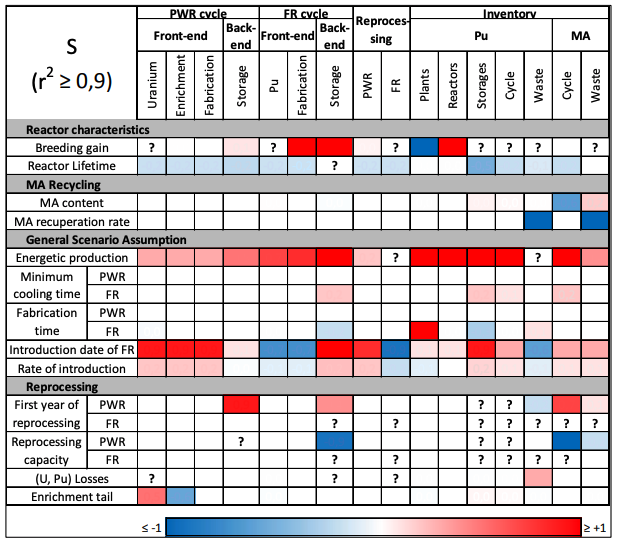
\includegraphics[scale=0.6]{./figures/oecd-sensitivitytable.png}
	\end{center}	
        \caption{Overall results from OECD one-at-a-time sensitivity analysis 
        study. Sensitivity Table with an overview of each output parameter's 
        sensitivity to the respective input parameters 
        \cite{noauthor_effects_2017}.}
	\label{fig:oecd-sensitivitytable}
\end{figure}

\begin{figure}[]
	\begin{center}
		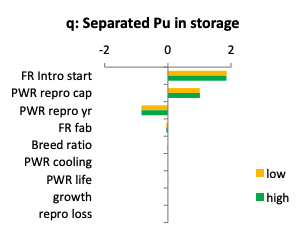
\includegraphics[scale=0.75]{./figures/oecd-tornado.png}
	\end{center}	
		\caption{A tornado plot from the OECD one-at-a-time sensitivity analysis 
        study, showing the sensitivity of the separated Pu in 
		storage amount to each input parameter \cite{noauthor_effects_2017}.}
	\label{fig:oecd-tornado}
\end{figure}

\subsection{Synergistic Sensitivity Analysis}
The synergistic sensitivity analysis technique involves multi-parameter 
input sweeps to view how synergistically changing input variables 
impacts the performance metrics.  
Synergistic sensitivity analysis is conducted by varying 
two input variables simultaneously and viewing their 
combined impact on each performance metric or a combination 
of weighted performance metrics. 
Figure \ref{fig:passerini_payoff} shows an example of this analysis 
in which thermal reprocessing and fast reactor technology 
introduction dates were varied, and the plot shows an objective 
payoff surface representing a combination of multiple performance 
metrics. 
Synergistic studies inform on the how variation in 
two input variables impacts the system; however, it fails to inform 
on the global sensitivity of the system. 

\begin{figure}[]
	\begin{center}
		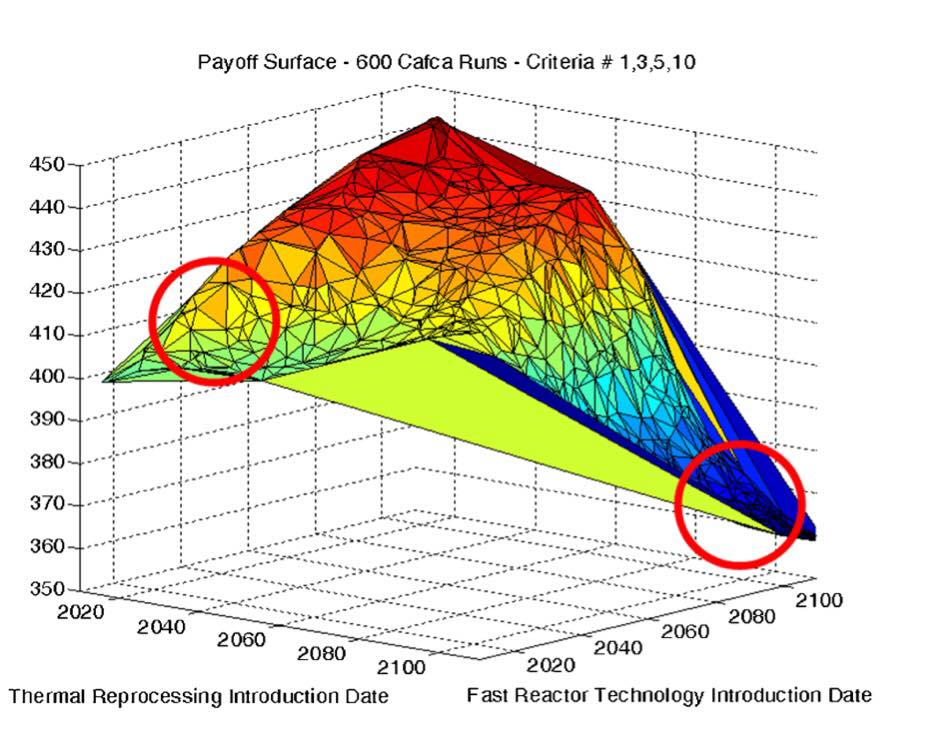
\includegraphics[scale=0.45]{./figures/passerini_payoff.jpg}
	\end{center}	
		\caption{Payoff surface for variation in thermal 
		reprocessing and fast reactor technology introduction date
		\cite{passerini_systematic_2014}}
	\label{fig:passerini_payoff}
\end{figure} 

\subsection{Global Sensitivity Analysis}
\label{sec:sobol}
To fully consider the synergistic effects of
simultaneous variation of all the input variables, a variance-based 
approach can be used instead \cite{thiolliere_methodology_2018}.
Thiolliere et al. conducted a global sensitivity analysis of a 
nuclear fuel cycle transition scenario by using Latin Hypercube sampling 
to generate Sobol indices. 
Sobol Indices provide the global sensitivity effect that each 
input variable has on a performance metric by decomposing the 
variance of the metric into fractions attributed to inputs or sets of inputs.
Essentially, it indicates which design parameter has 
the most influence on the response quantities.
A large Sobol index signifies that variation in that input 
variable is more impactful to the output parameter.

\subsection{Main Takeaways}
Sensitivity analysis studies of nuclear fuel cycles have previously been used to narrow 
down and compare a wide range of nuclear fuel cycle scenarios to determine 
the ideal scenario end types. 
The evaluation and screening study determined that the desired 
fuel cycle end states were EG23, EG24, EG29, and EG30.
These sensitivity analysis studies focused on high level input 
parameters such as reactor and reprocessing technologies, etc.
However, limited sensitivity studies have been performed to 
evaluate specific transition scenarios that describe the transition 
from the current to desired end states.
The only relevant sensitivity study was conducted by OECD 
\cite{noauthor_effects_2017}, however it was a basic one-at-a-time 
sensitivity analysis.   
Therefore, synergistic and global sensitivity analysis studies focused on
lower-level input parameters such as cooling time, 
introduction date of reprocessing/reactor 
technologies, the ratio of technology types should be conducted to 
understand the nuances brought about by the variation of low-level parameters. 
Through synergistic sensitivity analysis, these transition scenarios can be 
further optimized and used to inform other nuclear research areas 
such as reprocessing facility design, etc. 